\documentclass[10pt,twocolumn,letterpaper]{article}

% Use the official CVPR style when the author kit is present.  The fallback
% keeps this draft compilable before the CVPR 2027 kit is added.
\IfFileExists{cvpr.sty}{\usepackage[review]{cvpr}}{\usepackage[margin=0.75in,columnsep=0.25in]{geometry}}
\usepackage{times}
\usepackage{graphicx}
\usepackage{amsmath,amssymb}
\usepackage{booktabs}
\usepackage{multirow}
\usepackage{microtype}
\usepackage{xcolor}
\usepackage{url}
\usepackage{enumitem}

\newcommand{\method}{spatial serialization intervention}
\newcommand{\pp}{\,pp}
\newcommand{\ie}{i.e.,\ }
\newcommand{\eg}{e.g.,\ }

\title{Spatial Serialization Fragility in Dynamic-Resolution Vision-Language Models}
\author{Anonymous CVPR Submission}
\date{}

\begin{document}
\maketitle

\begin{abstract}
Dynamic-resolution vision-language models (VLMs) increasingly rely on visual-language interfaces that convert spatial evidence into variable-length token sequences, yet evaluations typically report accuracy under a single preprocessing realization.
We introduce \emph{evidence-preserving serialization invariance}---whether predictions remain consistent across controlled presentations of the same encoded visual evidence---as a reliability criterion for these interfaces, and define the Evidence-Preserving Serialization Gap (EPSG) to quantify relation-selective sensitivity.
Our post-encoder diagnostic counterfactuals reassign coherent spatial-region features and their associated interface-level position signals while holding source pixels, the question, the visual-feature multiset, and token count fixed.
Across LLaVA-OneVision-7B, Qwen2.5-VL-7B, and InternVL3-8B, we reveal task-selective instability: relational predictions are substantially less consistent under reserialization than object recognition.
A matched four-object recognition control shows no observed degradation in this sample, while binary relation accuracy falls from 93.75\% to 68.75\%.
The post-encoder decomposition reveals architecture-dependent content--position sensitivity patterns across Qwen and LLaVA.
Exhaustive four-region tests show that preserving a simple 2D adjacency graph is not sufficient for robustness, and unweighted voting over serializations does not provide a remedy.
These results identify an overlooked reliability dimension of the visual-language interface; they do not imply a generic token-order law, a universal VLM failure, or that dynamic resolution itself is the cause.
\end{abstract}

\section{Introduction}

Modern VLM pipelines follow a common path: image $\rightarrow$ visual encoding $\rightarrow$ visual tokens $\rightarrow$ language model.
Dynamic-resolution VLMs provide a practical and widely used setting in which this visual-language interface is explicit: LLaVA-OneVision inherits AnyRes-style global and local views~\cite{li2024llavaonevision}, Qwen2.5-VL uses a native dynamic-resolution vision encoder with multidimensional rotary position encoding~\cite{bai2025qwen25vl}, and InternVL-family models use dynamic high-resolution processing~\cite{chen2024internvl}.
Across these systems, region-to-slot assignment, grouping, separators, and interface-level position signals determine how two-dimensional evidence is delivered to the language model.
These choices are often treated as implementation details; however, if two interfaces preserve the same encoded evidence yet produce different relational predictions, serialization is part of the model's effective behavioral specification.
We do not attribute such differences to dynamic resolution itself; these models provide a setting in which to characterize this interface-level reliability property.

Most VLM evaluations report answer accuracy under a single preprocessing realization: one resizing, tiling, packing, and interface path.
This measures performance conditional on one interface realization while leaving unmeasured whether predictions remain consistent across justified alternatives that preserve visual evidence and task semantics.
This consistency gap is an evaluation blind spot: single-path accuracy cannot reveal whether the interface representation itself is behaviorally stable.
Prior analyses have documented hallucination, weak visual grounding, and spatial-reasoning deficits~\cite{tong2024eyes,chen2024spatialvlm}, while controlled benchmarks such as CLEVR, GQA, and SpatialSense isolate different forms of visual reasoning~\cite{johnson2017clevr,hudson2019gqa,yang2019spatialsense}.
Our question is therefore not simply whether a VLM can answer spatial questions, but whether its answers remain stable when the same evidence is represented through controlled alternative serializations.
We call this complementary reliability property \emph{evidence-preserving serialization invariance}.
Unlike generic token-permutation analyses, our principal diagnostic interventions occur after visual encoding while preserving source pixels, the selected feature multiset, question content, and visual-token count; they do not arbitrarily corrupt the sequence.
By contrast, arbitrary edits to a language sequence can change meaning, while ordinary crop-order tests can confound serialization with changes in encoder computation or position information.

We ask: \emph{Are relational predictions in dynamic-resolution VLMs invariant to alternative spatial serializations of the same visual evidence?}
We treat an image-to-sequence mapping as an interface whose visual content and position assignment can be intervened on separately after the vision encoder.
The intervention preserves the source image and post-encoder feature multiset while changing which spatial-region features occupy which sequence slots, which position values are assigned to those slots, or both.
Because architectures expose different visual-language interfaces, we instantiate the interventions along each model's native pathway while enforcing the same controlled invariants wherever the pathway permits.
This is an invariance test over the visual-language interface, rather than a claim about arbitrary sequence transformations.
The scientific question is whether controlled, evidence-preserving presentations of spatial regions selectively change relational behavior, and whether the observed sensitivity is shared across architectures.

Our empirical analysis characterizes serialization invariance as limited in the evaluated settings.
Behavioral reserialization effects appear in three tested model families, but the controlled post-encoder decomposition differs sharply between Qwen and LLaVA.
Recognition shows much smaller degradation than binary and compositional relations; this gap persists when recognition uses the same four-object scenes and distractors.
At the same time, a generic language-order perturbation is more destructive than the tested visual perturbation, so we do not claim that visual serialization is uniquely sensitive among all sequence operations.

Our contributions are threefold:
\begin{enumerate}[leftmargin=*,itemsep=1pt,topsep=2pt]
    \item We introduce evidence-preserving serialization invariance as a reliability criterion for visual-language interfaces and define EPSG to quantify task-selective serialization sensitivity.
    \item We provide controlled cross-model evidence that relational reasoning exhibits substantially larger serialization gaps than object recognition under the same visual evidence, including a matched four-object control with the same images and distractors.
    \item We reveal architecture-dependent serialization sensitivity patterns: Qwen and LLaVA exhibit different content--position coordination behaviors rather than one shared explanation across the tested architectures.
\end{enumerate}

\begin{figure*}[t]
    \centering
    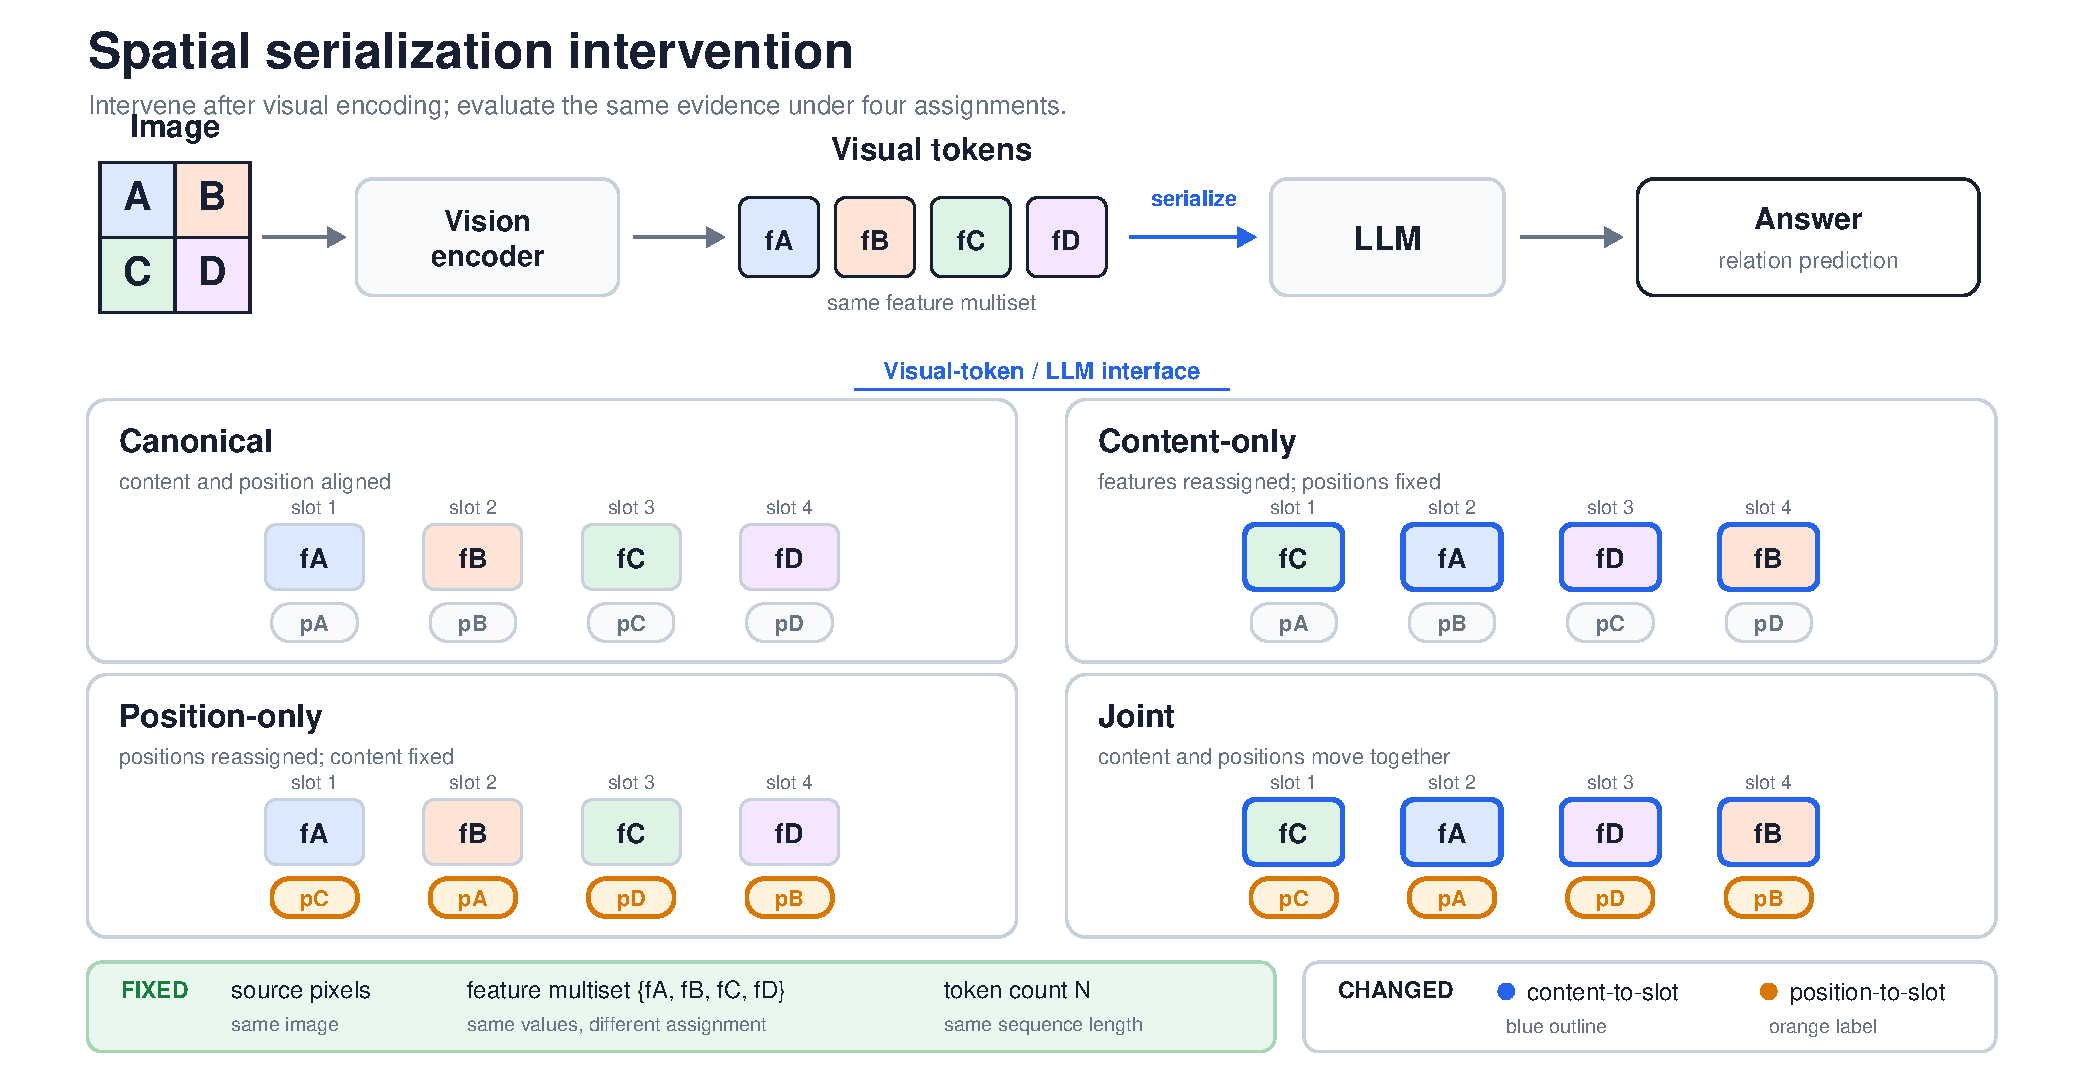
\includegraphics[width=0.97\textwidth]{figures/method_overview.pdf}
    \caption{\textbf{Spatial serialization intervention.}
    An image is encoded into visual features and then serialized for the language model.
    Canonical inference aligns region content with its native position assignment.
    Content-only reassigns regional features while positions remain fixed; position-only reassigns positions while content remains fixed; joint moves both together.
    The source pixels, selected feature multiset, and token count are fixed in all post-encoder conditions.
    Model-specific tokens that remain fixed are detailed in Sec.~\ref{sec:instantiation}.}
    \label{fig:overview}
\end{figure*}

\section{Related Work}

\paragraph{Dynamic resolution and visual token sequences.}
Vision Transformers make image processing explicitly sequential by flattening patch embeddings and combining them with position information~\cite{dosovitskiy2021vit}.
Subsequent designs process variable resolutions and aspect ratios by packing variable-length patch sequences~\cite{dehghani2023navit}, resampling visual inputs~\cite{alayrac2022flamingo}, or combining global and local views.
Modern open VLMs instantiate these choices differently: LLaVA-OneVision uses AnyRes-style processing~\cite{li2024llavaonevision}, Qwen2.5-VL uses a native visual grid and M-RoPE~\cite{bai2025qwen25vl}, and InternVL provides another high-resolution model family~\cite{chen2024internvl}.
Prior work has improved capacity, efficiency, or transfer under a chosen tokenization.
We instead characterize whether predictions are invariant to controlled alternatives at the resulting visual-token interface.

\paragraph{Order and position as model variables.}
Patch size, token selection, and packing are known design variables rather than implementation-neutral details~\cite{beyer2023flexivit,dehghani2023navit}.
Patch-order permutation has also been used as a training signal for object-centric autoregressive vision models~\cite{kakogeorgiou2024spot}.
The closest reliability studies examine position bias when multiple images are reordered~\cite{tian2025positionbias}.
Our setting differs in acting \emph{within one image}: we move coherent spatial-region features among visual sequence slots and, for Qwen and LLaVA, separately intervene on the position values delivered to the language model.
We do not infer an internal circuit from attention maps; the evidence in this paper is behavioral and interventional at a specified interface.

\paragraph{Spatial reasoning diagnostics.}
CLEVR and GQA use controlled programs or scene graphs to diagnose compositional visual reasoning~\cite{johnson2017clevr,hudson2019gqa}, while SpatialSense reduces simple geometric and language shortcuts in real images~\cite{yang2019spatialsense}.
Recent studies document persistent spatial and basic-perception limitations in VLMs~\cite{chen2024spatialvlm,tong2024eyes}.
Our synthetic scenes inherit the diagnostic logic of controlled datasets but target a different variable: the semantic scene and question stay fixed while the visual-language interface changes.
The goal is not a broader spatial benchmark; it is controlled isolation of serialization sensitivity.

\section{Spatial Serialization Intervention}
\label{sec:method}

\subsection{Problem formulation}

Let a vision encoder and projector produce visual features $F=(f_1,\ldots,f_N)$, $f_i\in\mathbb{R}^{d}$, with position-related signals $P=(p_1,\ldots,p_N)$.
Given a question $q$, the model output and a diagnostic serialization transformation are written as
\begin{align}
    y &= M\!\left(\mathcal{S}(F,P),q\right), \\
    \mathcal{S}(F,P) &\longrightarrow \mathcal{S}'(F,P).
\end{align}
Here $\mathcal{S}$ serializes visual content and position information at the visual-language interface, and $P$ denotes signals exposed at this interface rather than necessarily the encoder's internal 2D positions.
The arrow denotes a controlled diagnostic transformation used to test behavioral stability, not an assumption that the two serialized inputs are equivalent to the model.
The visual evidence remains fixed: the source image and selected visual-feature multiset are unchanged; the question and token count are also fixed.
Let $\mathcal{E}$ denote the family of such evidence-preserving serializations.
For $\mathcal{S},\mathcal{S}'\in\mathcal{E}$, prediction-level serialization invariance on an example requires
\begin{equation}
    M\!\left(\mathcal{S}(F,P),q\right)=M\!\left(\mathcal{S}'(F,P),q\right).
\end{equation}
For a permutation $\pi$ over coherent region blocks, define $\pi(F)$ and $\pi(P)$ as blockwise reassignment to destination slots.
The four conditions are
\begin{align}
    \text{canonical:}      &\quad \mathcal{S}(F,P), \\
    \text{content-only:}   &\quad \mathcal{S}(\pi(F),P), \\
    \text{position-only:}  &\quad \mathcal{S}(F,\pi(P)), \\
    \text{joint:}          &\quad \mathcal{S}(\pi(F),\pi(P)).
\end{align}
The selected content multiset and position-value multiset are preserved.
Content-only changes the mapping from region features to sequence slots; position-only changes which position values those features receive; joint preserves the pairing between each moved feature and its moved position while relocating both.
Figure~\ref{fig:overview} summarizes the construction.

These diagnostic counterfactuals are not proposed inference procedures.
They serve as a controlled lens on the visual-language interface: by fixing source pixels, the question, the selected feature multiset, and token count, they test behavioral stability under specified serialization changes without presuming that all serializations are semantically equivalent.

\subsection{Quantifying Serialization Fragility}

Let $\mathcal{S}_{\mathrm{can}}$ denote canonical serialization and $\mathcal{S}_{\mathrm{int}}$ an evidence-preserving intervention.
For task $t$, define its serialization sensitivity and the Evidence-Preserving Serialization Gap as
\begin{align}
    \Delta_t &= \operatorname{Acc}_t(\mathcal{S}_{\mathrm{can}})-\operatorname{Acc}_t(\mathcal{S}_{\mathrm{int}}), \\
    \mathrm{EPSG} &= \Delta_{\mathrm{relation}}-\Delta_{\mathrm{recognition}}.
\end{align}
A positive EPSG indicates that serialization changes degrade relational accuracy more than recognition accuracy; we compute it separately for binary and compositional relations.
Recognition is used as a matched capability control because it tests whether serialization changes primarily affect relational composition rather than basic visual identification.
Unlike raw accuracy degradation, EPSG measures whether serialization sensitivity is selective to relational reasoning after accounting for matched recognition behavior.
EPSG is a diagnostic reliability measure, not a training objective or inference method.
Result tables retain their stated perturbed-minus-canonical sign convention.

\subsection{Controlled invariants}

For every post-encoder comparison, source image pixels, question, answer, model weights, tensor shape, visual-token count, and selected feature multiset are fixed; the position multiset is also fixed when positions are moved.
Thus a prediction change cannot be attributed to lower image resolution, missing image regions, fewer tokens, or a different set of encoded region features.

Some architecture-specific tokens remain canonical by design.
This makes the intervention conservative but partial: it targets comparable spatial blocks rather than every visual token.

\subsection{Model-specific instantiations}
\label{sec:instantiation}

\paragraph{Qwen2.5-VL.}
A $768\!\times\!768$ image produces a logged $1\!\times\!54\!\times\!54$ vision grid and a merged $27\!\times\!27$ language-model grid (729 visual tokens).
We move four $13\!\times\!13$ corner blocks after the vision encoder, for 676 intervened tokens; the center row and column remain fixed.
Content-only patches post-encoder image features, position-only patches all visual axes returned by Qwen's M-RoPE index construction, and joint applies the same block permutation to both.

\paragraph{LLaVA-OneVision.}
The packed visual sequence contains 729 global-thumbnail tokens and a $54\!\times\!55$ high-resolution matrix: 54 content tokens plus one newline token per row, for 3,699 visual tokens in total.
We move four $27\!\times\!27$ high-resolution content blocks (2,916 tokens) after feature projection.
The 729 thumbnail tokens and 54 newline tokens remain fixed.
The position intervention changes the language model's scalar sequence position IDs on the same visual slots; it does not modify the SigLIP encoder's internal positions.

\paragraph{InternVL3.}
The behavioral replication uses four row-major $384\!\times\!384$ crops plus a whole-image thumbnail, each resized to $448\!\times\!448$, with 1,280 recorded visual tokens.
Crop order is changed before model inference.
We do not implement the clean post-encoder content/position decomposition for InternVL and therefore use it only as evidence of behavioral transfer, not of a shared internal account.

\section{Experiments}
\label{sec:experiments}

\subsection{Experimental setup}

\paragraph{Controlled synthetic benchmark.}
We generate 440 scenes on $768\!\times\!768$ canvases.
Each relation image contains four 40-pixel colored shapes; the answer-critical pair has center distance 168 pixels and is accompanied by an aligned distractor pair.
Horizontal and vertical relations are balanced (220 scenes each).
We evaluate: (i) object recognition, (ii) binary relations (left/right/above/below), and (iii) compositional relations that require selecting the shape at a queried relation to a reference object.
The standard recognition item uses a separately rendered single target at the matched location; Sec.~\ref{sec:matched} adds a four-object matched control.
The synthetic design is intentional: it supports controlled isolation of serialization effects by fixing visual evidence, object identity, spatial configuration, visual-token count, and the specified serialization change.
It is not intended to approximate the full diversity of real-world images, and broader natural-image validation remains important.

\paragraph{Models and inference.}
We use LLaVA-OneVision-7B in FP16, Qwen2.5-VL-7B in BF16, and InternVL3-8B in BF16, each at an immutable checkpoint revision listed in the supplement.
Inference uses greedy decoding, batch size one per worker, and at most eight new tokens on four independent RTX~4090 workers.
LLaVA, Qwen, and InternVL use 3,699, 729, and 1,280 recorded visual tokens, respectively, for the tested inputs.

\paragraph{Statistics.}
The independent unit is the scene.
We report accuracy changes in percentage points (pp), with 95\% percentile intervals from 20,000 scene-level bootstrap resamples.
Paired binary outcomes use a two-sided exact binomial test over discordant scene pairs.
Holm correction is applied within the prespecified comparison families for the intervention, natural, topology, and ensemble analyses.
E17--E19 reuse the same 192-scene prediction set and are not independent replications.

\subsection{RQ1: How sensitive is relational reasoning to spatial serialization?}
\label{sec:crossmodel}

\subsubsection{Cross-model evidence}
Because VLM architectures expose different visual-language interfaces, cross-model comparisons are interpreted as behavioral evidence of serialization sensitivity rather than identical causal decompositions.
We first ask whether behavioral sensitivity is confined to one model.
For LLaVA and InternVL, we compare canonical and permuted local-crop order within the cross-tile condition.
For Qwen, the corresponding initial test permutes native-grid patch quadrants before the vision encoder.
These architecture-specific perturbations preserve image content, question, answer, and token count; only the post-encoder experiments in Sec.~\ref{sec:decomp} additionally guarantee a fixed feature multiset.

Figure~\ref{fig:crossmodel} and Table~\ref{tab:crossmodel} show the paired changes.
LLaVA recognition changes by $-0.23\pp$, compared with $-35.45\pp$ for binary relations and $-26.59\pp$ for composition.
InternVL recognition shows a $0.00\pp$ change, while the relation tasks change by $-20.23\pp$ and $-9.32\pp$.
Qwen's pre-encoder native-grid perturbation also harms recognition ($-13.18\pp$), but its binary and compositional losses are larger ($-43.18\pp$ and $-56.36\pp$).
Thus sensitivity is present in all three evaluated families, but the initial Qwen test is not evidence-preserving after the encoder and motivates the cleaner decomposition below.

\begin{figure}[t]
    \centering
    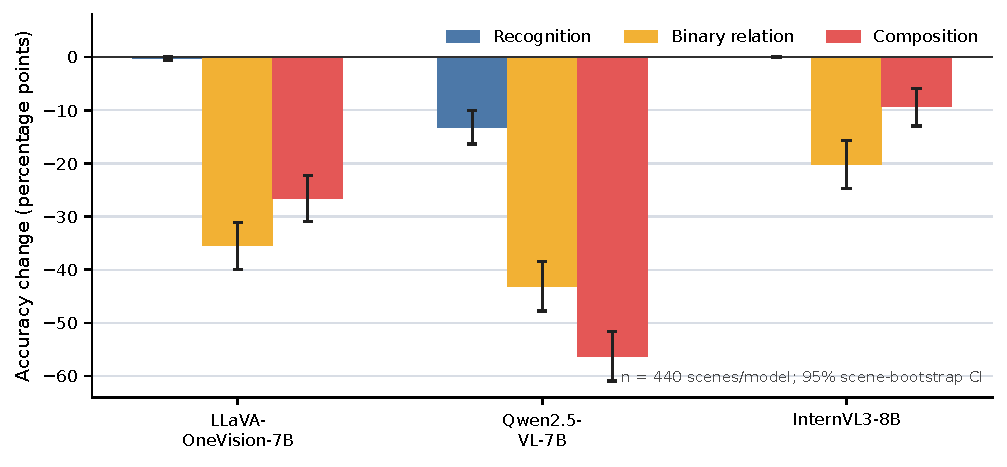
\includegraphics[width=\linewidth]{figures/cross_model_main.pdf}
    \caption{\textbf{Cross-model behavioral sensitivity.}
    Paired accuracy change under the primary reserialization contrast for 440 scenes per model; error bars are 95\% scene-bootstrap intervals.
    LLaVA and InternVL compare crop-order conditions within cross-tile inputs; Qwen uses a pre-encoder native-grid permutation.
    The latter changes encoder computation and is separated from the controlled post-encoder analysis.}
    \label{fig:crossmodel}
\end{figure}

\begin{table}[t]
\centering
\small
\setlength{\tabcolsep}{3.2pt}
\caption{\textbf{Cross-model reserialization effects} on 440 scenes/model. Values are perturbed minus canonical accuracy in pp, with 95\% scene-bootstrap CIs.}
\label{tab:crossmodel}
\begin{tabular}{lrrr}
\toprule
Model & Recognition & Binary & Composition \\
\midrule
LLaVA & $-0.23$ & $-35.45$ & $-26.59$ \\
 & $[-0.68,0]$ & $[-40.00,-31.14]$ & $[-30.91,-22.27]$ \\
InternVL & $0.00$ & $-20.23$ & $-9.32$ \\
 & $[0,0]$ & $[-24.77,-15.68]$ & $[-12.95,-5.91]$ \\
Qwen & $-13.18$ & $-43.18$ & $-56.36$ \\
 & $[-16.36,-10.00]$ & $[-47.73,-38.41]$ & $[-60.91,-51.59]$ \\
\bottomrule
\end{tabular}
\end{table}

\subsubsection{Matched recognition control}
\label{sec:matched}

The smaller observed recognition degradation could be dismissed as a consequence of an easier, single-object task.
We therefore evaluate 96 of the same four-object scenes with the question ``What shape is the \emph{color} object?''
The target color is unique; the model must locate one object among three distractors and bind its color to its shape, but it need not evaluate a spatial relation.
The image, four objects, distractors, feature multiset, 3,699-token count, and position IDs are identical between canonical and LLaVA content-only conditions.

Matched recognition is 100\% in both conditions, whereas binary relation accuracy falls from 93.75\% to 68.75\%, a $25.00\pp$ degradation (95\% CI $[16.67,33.33]$; exact paired $p=1.19\!\times\!10^{-7}$).
The corresponding difference-in-differences, or EPSG, is $25.00\pp$.
This result addresses distractor and image-complexity mismatch, although the recognition task remains at ceiling and does not equalize every reasoning operation.

\begin{figure}[t]
    \centering
    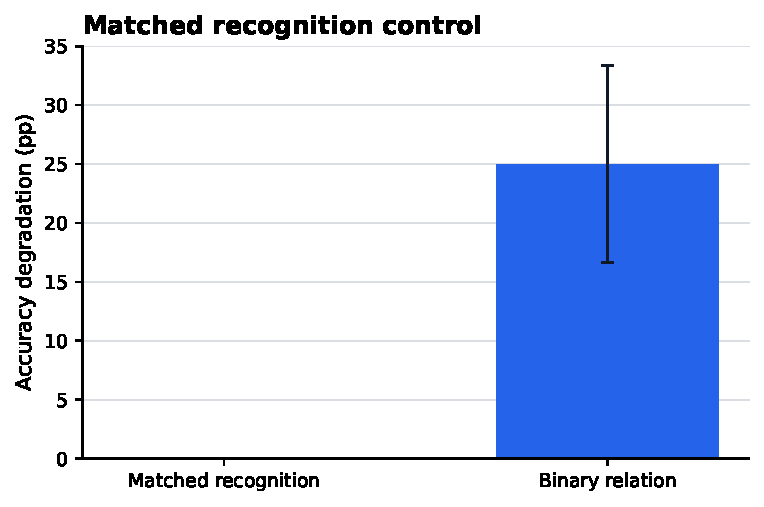
\includegraphics[width=0.94\linewidth]{figures/matched_recognition_control.pdf}
    \caption{\textbf{Matched four-object recognition control.}
    Accuracy degradation under LLaVA post-encoder content permutation on 96 scenes.
    Recognition uses the same four-object image and distractors as the relation task.
    Error bars show 95\% scene-bootstrap intervals.}
    \label{fig:matched}
\end{figure}

\subsubsection{Controlled-natural validation}
\label{sec:natural}

To reduce dependence on geometric icons, we construct a held-out benchmark from COCO 2017 object instances~\cite{lin2014coco}.
Two category-distinct object crops are placed on a controlled $768\!\times\!768$ canvas at a 200-pixel center distance.
A red frame marks the target and a blue frame marks the reference.
The 28-scene calibration set and 108-scene test set have disjoint COCO source-image IDs; the test contains 972 model inputs.
We use conditional candidate likelihoods rather than free-form generation.

Within the held-out test, moving from canonical cross-tile serialization to the permuted version changes recognition by $0.00\pp$ (95\% CI $[0,0]$), binary relations by $-21.30\pp$ ($[-29.63,-13.89]$, Holm $p=7.15\!\times\!10^{-7}$), and composition by $-8.33\pp$ ($[-14.81,-2.78]$, Holm $p=.0234$).
The cross-tile condition itself is not worse than the same-tile condition for either relation task, independently rejecting a universal boundary penalty.
This experiment is controlled-natural evidence, not a test on intact, unconstrained scenes: it uses composed object crops and colored role markers, and the compositional calibration threshold is passed by one example.

\subsection{RQ2: How do content and position assignments contribute across architectures?}
\label{sec:decomp}

We next isolate interface variables after the vision encoder using the four conditions in Sec.~\ref{sec:method}.
Each model is evaluated on 440 scenes and 5,280 model inputs.
The destination-to-source region permutation is $(2,0,3,1)$.

The two models exhibit different profiles (Fig.~\ref{fig:decomp}; Table~\ref{tab:decomp}).
For Qwen, recognition is 100\% under both canonical and content-only conditions, while binary accuracy decreases by $8.41\pp$ and composition by $22.50\pp$.
Position-only movement is null for binary relations and changes composition by only $-0.23\pp$ with an interval containing zero.
Moving content and M-RoPE coordinates jointly resembles content-only movement.
These results reject a simple M-RoPE-coordinate mismatch as a sufficient account for Qwen in this setting.

LLaVA behaves differently.
Moving content alone changes binary and compositional accuracy by $-35.45\pp$ and $-26.59\pp$; moving language-model positions alone changes them by $-32.27\pp$ and $-33.41\pp$.
Joint movement reduces the losses to $-6.36\pp$ and $-4.32\pp$.
The content-by-position interactions are $+61.36\pp$ for binary relations and $+55.68\pp$ for composition.
The joint compositional effect itself does not survive the full 18-comparison Holm family ($p_{\mathrm{adj}}=.177$).
LLaVA therefore depends strongly on content--position consistency, whereas Qwen is dominated by content-to-slot assignment.

\begin{figure*}[t]
    \centering
    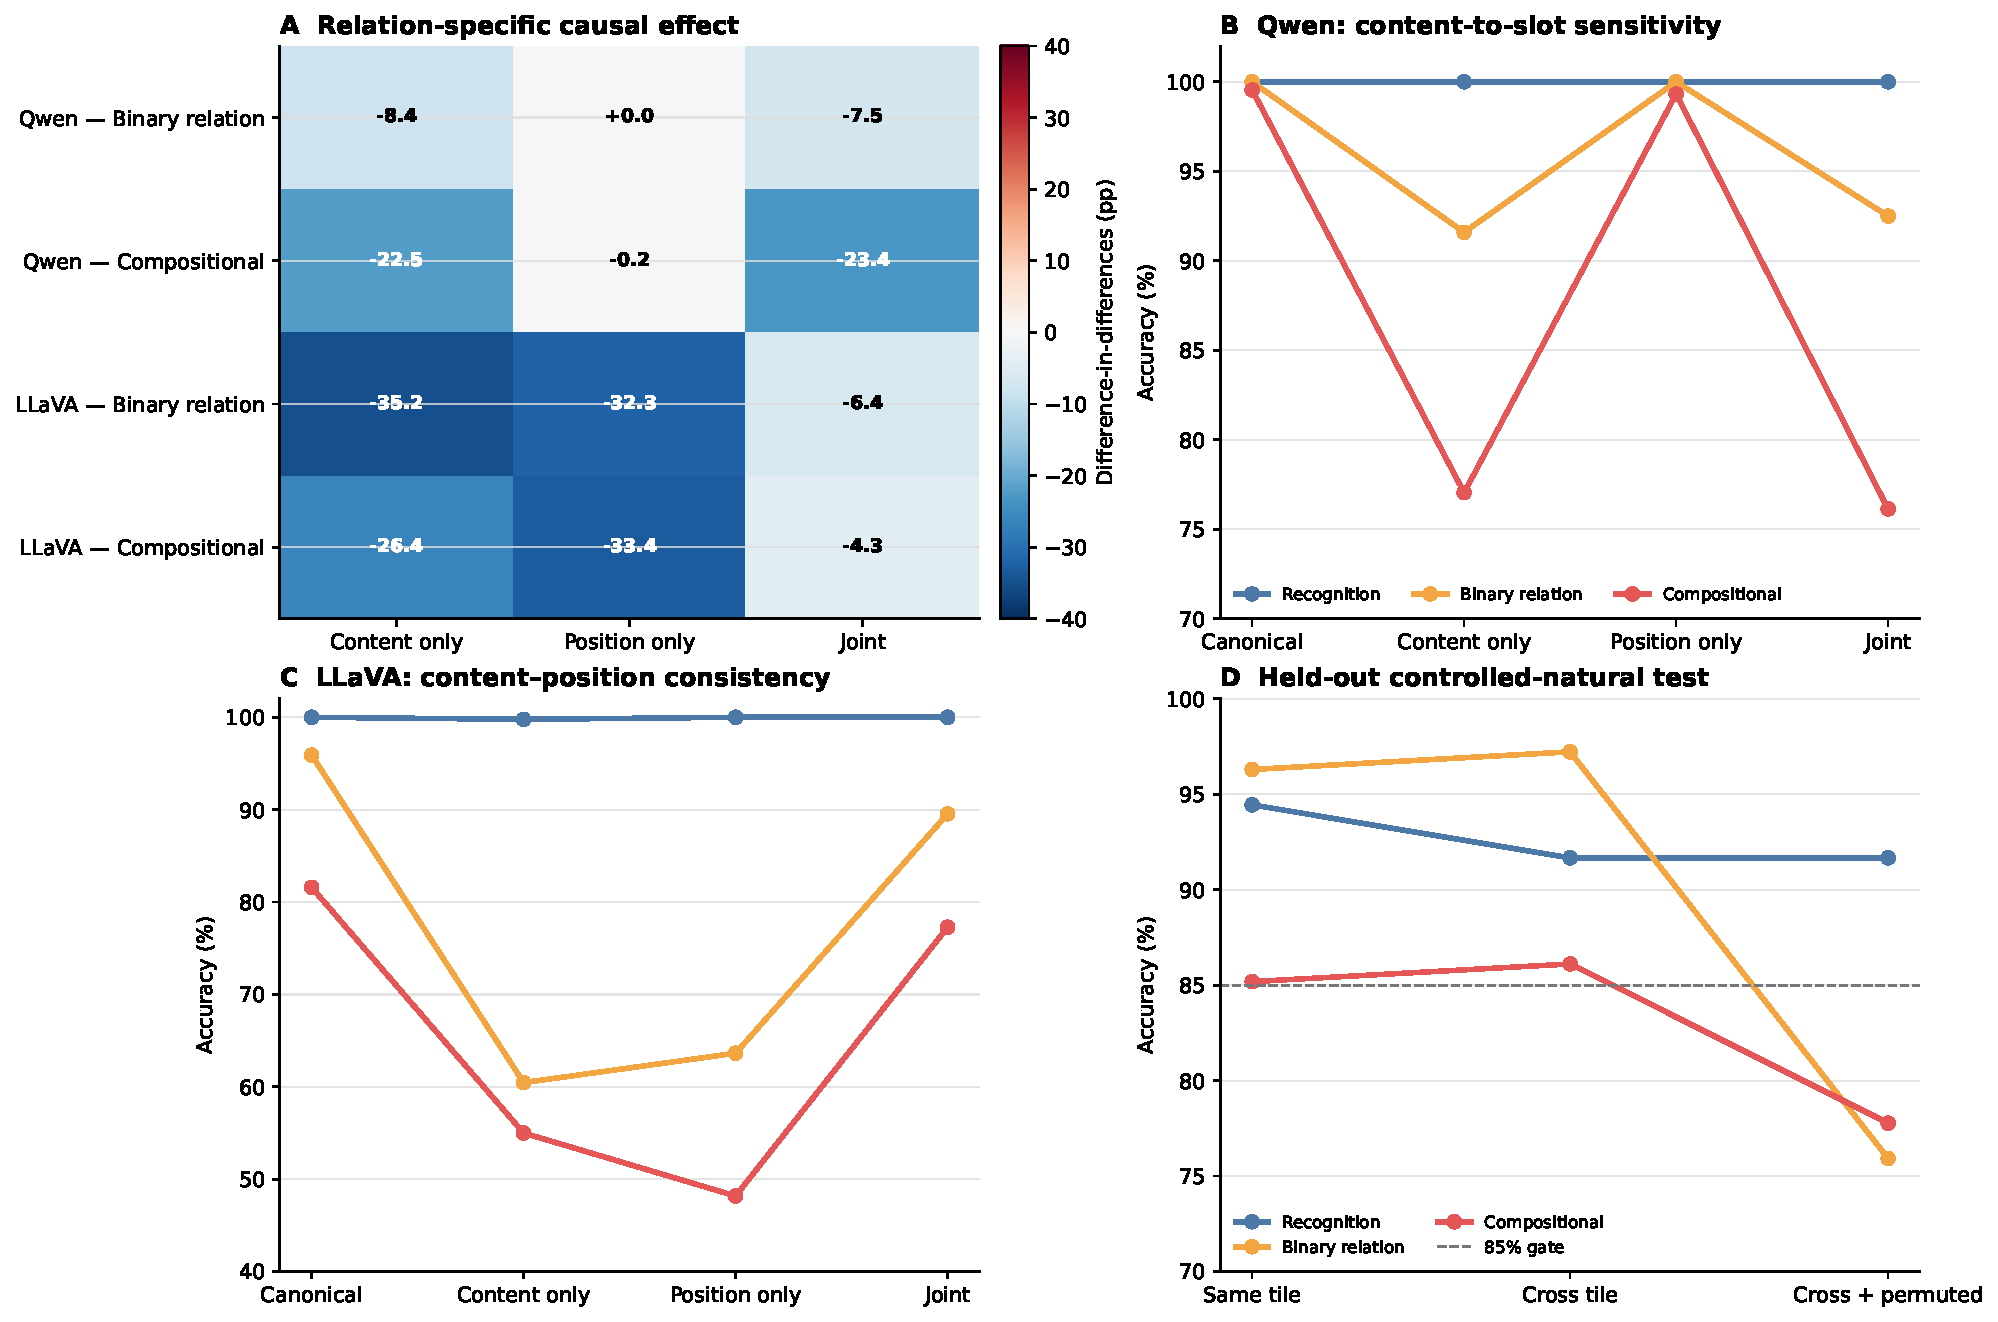
\includegraphics[width=0.96\textwidth]{figures/final_validation.pdf}
    \caption{\textbf{Post-encoder decomposition and controlled-natural validation.}
    Qwen (top right) is primarily sensitive to content-to-slot assignment; LLaVA (bottom left) is harmed by moving content or language-model positions alone and largely recovers when they move together.
    The left heatmap reports relation-specific changes relative to the recognition control.
    On 108 held-out controlled COCO-crop compositions (bottom right), reserialization changes relation accuracy but not recognition.
    These inputs are composed object crops with colored role markers, not unmodified full photographs.}
    \label{fig:decomp}
\end{figure*}

\begin{table}[t]
\centering
\small
\setlength{\tabcolsep}{3.5pt}
\caption{\textbf{Post-encoder change from canonical} (pp) on 440 scenes/model. All recognition changes are between $0$ and $-0.23\pp$.}
\label{tab:decomp}
\begin{tabular}{llrr}
\toprule
Model & Intervention & Binary & Composition \\
\midrule
Qwen & Content & $-8.41$ & $-22.50$ \\
 & Position & $0.00$ & $-0.23$ \\
 & Joint & $-7.50$ & $-23.41$ \\
\midrule
LLaVA & Content & $-35.45$ & $-26.59$ \\
 & Position & $-32.27$ & $-33.41$ \\
 & Joint & $-6.36$ & $-4.32$ \\
\bottomrule
\end{tabular}
\end{table}

\subsection{RQ3: How well do existing spatial explanations account for the observed sensitivity?}
\label{sec:falsification}

\paragraph{Does preserving 2D adjacency explain robustness?}
For 192 balanced scenes per model, we exhaust all 24 permutations of four regions and move content and positions jointly after the encoder.
Seven nonidentity transformations preserve the unweighted 2$\times$2 grid-adjacency graph; sixteen break it.
Breaking-minus-preserving contrasts are small and include zero for LLaVA binary ($+0.61\pp$), LLaVA composition ($+0.99\pp$), Qwen binary ($-0.26\pp$), and Qwen composition ($-1.22\pp$); all Holm-adjusted $p\geq .115$.
Yet graph-preserving transformations are associated with losses as large as $21.35\pp$ for LLaVA composition and $24.48\pp$ for Qwen composition.
Simple 2D adjacency preservation is therefore not sufficient on this topology.

\paragraph{Is this uniquely a visual-order effect?}
On a 96-scene LLaVA subset, we compare the visual content permutation with a matched four-block permutation of non-visual query embeddings.
The language perturbation changes word order and therefore is not semantics preserving, but it keeps prompt length and the embedding multiset fixed.
It is more destructive than visual reserialization: binary/compositional losses are $51.04/69.79\pp$ for language order versus $25.00/25.00\pp$ for visual order.
Consequently, we do not claim that visual serialization is uniquely sensitive compared with generic transformer sequence perturbations.
Its relevance is that the visual intervention changes relational outputs while preserving image and query semantics.

\subsection{RQ4: How effective are simple inference-time mitigation strategies?}

\paragraph{Five-view voting.}
We reuse the same predictions for canonical, 180-degree reversal, 90-degree rotation, column-major, and one fixed topology-breaking view.
Unweighted modal voting with canonical tie breaking improves no task.
It changes LLaVA binary/compositional accuracy by $-3.13/-0.52\pp$ and Qwen by $-6.25/-5.73\pp$; the two Qwen losses remain significant after Holm correction.
This is a negative result for one simple ensemble, not evidence against learned or calibrated selection.

\begin{figure*}[t]
\centering
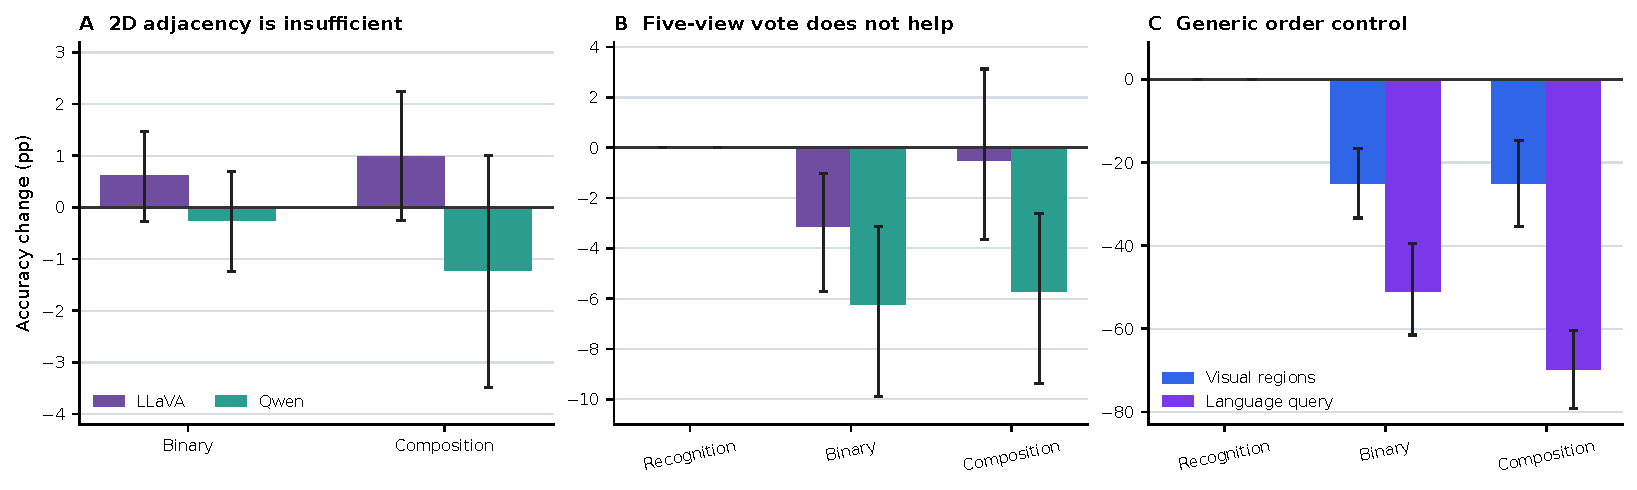
\includegraphics[width=0.98\textwidth]{figures/falsification_main.pdf}
\caption{\textbf{Falsification analyses.}
(A) Primary adjacency-breaking minus adjacency-preserving contrasts include zero for both relation tasks and models.
(B) Unweighted voting over five fixed serializations does not improve canonical inference; this analysis reuses the topology predictions.
(C) A non-semantic-preserving language-query permutation is more destructive than visual-region reserialization, so the results do not establish unique visual-order sensitivity.
Bars show paired accuracy changes and error bars show 95\% scene-bootstrap intervals.}
\label{fig:falsification}
\end{figure*}

\section{Analysis and Discussion}

\paragraph{The effect is relation selective, while recognition is comparatively more stable.}
Across the clean Qwen and LLaVA interventions, recognition changes by at most $0.23\pp$ while relation losses reach tens of percentage points.
The matched four-object control rules out the narrow explanation that the recognition result follows only from an isolated-object image.
The held-out controlled-natural set also has below-ceiling recognition, with 91.67\% accuracy in both compared conditions and an observed change of $0.00\pp$.
Nevertheless, many synthetic recognition cells are at 100\%, so we interpret the result as substantially greater stability, not proof of universal recognition invariance.

\paragraph{There is no single content/position sensitivity pattern.}
Qwen's position-only result is nearly null and joint movement remains as harmful as content-only movement.
LLaVA shows the opposite interaction pattern: either isolated content or isolated position movement is harmful, while moving them consistently is largely protective.
InternVL provides behavioral replication but lacks the corresponding post-encoder decomposition.
The appropriate cross-model conclusion is therefore an architecture-dependent interface sensitivity that cannot be reduced to a single content/position sensitivity pattern across the tested architectures.

\paragraph{Tile boundaries are not the headline.}
The original hypothesis concerned whether answer-critical objects cross a crop boundary.
The final evidence rejects this as a universal account: LLaVA's canonical binary accuracy improves in the cross-tile condition, its canonical compositional effect includes zero, and the controlled-natural relation scores do not decline at the boundary.
InternVL does show a negative boundary effect, and LLaVA's factorial analysis finds interactions among partition, order, and thumbnail content.
Boundary placement can therefore modulate behavior, but the robust shared phenomenon is sensitivity to the serialization interface.

\paragraph{Why this matters.}
Visual preprocessing and token serialization are often treated as engineering details outside the model.
Our results show that they should instead be considered part of a VLM's effective behavioral specification: two interfaces containing the same encoded evidence can induce different relational answers.
A score obtained under one preprocessing realization therefore does not fully specify behavior when region-to-sequence assignment can change the result.
This matters for model comparison, deployment, and reproducibility.
At minimum, dynamic-resolution evaluations should specify the serialization policy and include invariance checks when the task depends on spatial composition.

\section{Limitations}

This study has four central limitations.
First, it does not identify a unique internal neural process.
The interventions hold other specified factors fixed while varying content and position assignments at the visual-token/language-model interface, but they do not locate a circuit, explain how training creates the sensitivity, or justify a claim about attention-mediated binding.

Second, controlled synthetic scenes are deliberate: they isolate serialization effects by fixing visual evidence, object identity, spatial configuration, token count, and the specified transformation.
This control narrows ecological validity, and our COCO-derived benchmark uses composed object crops and colored markers rather than intact photographs.
A 60-scene VSR subset was directionally consistent but had near-chance canonical performance and a nonsignificant exact paired test, so it is not used as confirmatory evidence.
Broader validation on unconstrained natural images remains future work.

Third, the post-encoder intervention is architecture specific and partial.
The LLaVA thumbnail and newline tokens and the Qwen center row and column remain fixed.
The InternVL experiment changes crop order before encoding and lacks the same decomposition.
We evaluate one resolution, primarily a 2$\times$2 region layout, three open model families, and a narrow set of spatial/compositional tasks.
We do not establish that dynamic resolution is necessary relative to a matched fixed-resolution architecture.

Fourth, we do not demonstrate a mitigation.
Unweighted voting fails, overlap and coordinate-prompt probes are setting dependent, and no training-time objective is tested.
Future work should evaluate intact natural scenes with sufficiently strong canonical baselines, larger and multiscale region graphs, additional architectures, and training procedures that explicitly encourage serialization consistency.

\section{Conclusion}

We show that evidence-preserving serialization invariance is an important reliability dimension for the visual-language interfaces of dynamic-resolution VLMs.
Across the evaluated models and tasks, relational predictions are substantially more fragile than recognition under controlled reserialization, even when source pixels, the post-encoder feature multiset, the question, and token count are fixed.
The tested architectures exhibit different content--position sensitivity patterns, while preserving simple 2D adjacency or applying unweighted serialization voting does not ensure relational consistency.
Together, these findings establish that interface serialization is part of the evaluated VLM system rather than merely an implementation detail, without attributing the observed fragility to dynamic resolution itself or to a single shared internal process.
Future work should study training-time robustness objectives and serialization-aware architectures that improve relational consistency across justified, evidence-preserving interface transformations.
More broadly, serialization behavior should be considered part of a VLM's behavioral specification rather than merely an engineering detail.

{\small
\IfFileExists{ieeenat_fullname.bst}{\bibliographystyle{ieeenat_fullname}}{\bibliographystyle{plain}}
\bibliography{references}
}

\end{document}
